%% AIAA Journal Paper Template for Lab Report
\documentclass[conf]{new-aiaa}

% Package Imports
\usepackage{csvsimple}
\usepackage{graphicx}
\usepackage{amsmath, amssymb}
\usepackage{siunitx}
\usepackage{listings}
\usepackage{booktabs}
\usepackage{float}
\usepackage[utf8]{inputenc}
\usepackage{listings}
\usepackage{float}
\usepackage{graphicx}
\usepackage{amsmath}
\usepackage[version=4]{mhchem}
\usepackage{siunitx}
\usepackage{longtable,tabularx}
\setlength\LTleft{0pt} 

% Title & Author
\title{Dynamic Pressure and Airspeed Measurements in a Low-Speed Wind Tunnel}
\author{Parham Khodadi\footnote{Aerospace Engineering student, San Diego State University}}
\affil{A E 303, Section 3, with Dr. Xiaofeng Liu}

\begin{document}

\maketitle

\begin{abstract}
This experiment investigates the uniformity of the flow field in a low-speed wind tunnel using a total pressure rake. The study examines the configuration and operating principles of the wind tunnel while applying Bernoulli’s equation to determine dynamic pressure and velocity measurements in free-stream conditions. Additionally, a contour map is utilized to visualize the two-dimensional streamwise velocity distribution across the test section.

\end{abstract}

\section{Nomenclature}

{\renewcommand\arraystretch{1.0}
\noindent\begin{longtable*}{@{}l @{\quad=\quad} l@{}}
$q$ & Dynamic pressure (Pa) \\
$\bar{q}$ & Mean dynamic pressure (Pa) \\
$V$ & Airspeed (m/s) \\
$\bar{V}$ & Mean airspeed (m/s) \\
$\rho$ & Air density (kg/m$^3$) \\
IAS & Indicated Airspeed (m/s) \\
$p_0$ & Total pressure (Pa) \\
$p_s$ & Static pressure (Pa) \\
$Re$ & Reynolds number \\
$\mu$ & Dynamic viscosity of air (Pa·s) \\
$q_mean$ & Mean dynamic pressure (Pa) \\
$V_\infty$ & Freestream velocity (m/s) \\
$T$ & Temperature (K or °C) \\
$P_{ambient}$ & Ambient pressure (Pa or inHg) \\
$\rho_\infty$ & Freestream air density (kg/m³) \\
$\Delta p$ & Pressure differential (Pa) \\



\end{longtable*}}

\section{Introduction}

Flow uniformity in a wind tunnel test section is crucial for reliable aerodynamic testing. This experiment evaluates dynamic pressure and airspeed variations using a Pitot tube rake in the SDSU low-speed wind tunnel.

Total and static pressures were recorded at three test conditions (0, 2, and 5 inH2O), and airspeed was computed using Bernoulli’s equation. A convergence test determined the number of samples required for stable time-averaged pressure measurements, with a threshold of 0.005\%.

The results provide insight into test section uniformity, measurement stability, and wind tunnel performance.


\section{Theory}

\subsection{Velocity Measurement Using Pitot Tubes}
The uniformity of flow in a wind tunnel test section is essential for reliable aerodynamic testing. A Pitot tube rake is used to measure total pressure, while a separate static pressure probe (Port 7) provides a reference static pressure, assuming negligible lateral pressure gradients. Velocity is determined using Bernoulli’s equation:

\begin{equation}
    V = \sqrt{\frac{2q}{\rho}}
\end{equation}

where the dynamic pressure \( q \) is:

\begin{equation}
    q = p_0 - p_s
\end{equation}

where \( p_0 \) is total pressure, \( p_s \) is static pressure, and \( \rho \) is air density. The same calculation is applied at the test section inlet using a separate Pitot tube (Ports 61 \& 62) to determine the Indicated Airspeed (IAS).

\subsection{Flow Uniformity and Data Reduction}
To assess flow uniformity, deviations from the mean dynamic pressure \( \bar{q} \) are computed as:

\begin{equation}
    \frac{q - \bar{q}}{\bar{q}} \times 100\%
\end{equation}

Similarly, airspeed deviations are evaluated as:

\begin{equation}
    \frac{V - \bar{V}}{\bar{V}} \times 100\%
\end{equation}

These calculations quantify test section non-uniformities and identify variations in airflow.

\subsection{Convergence Testing for Dynamic Pressure}
A convergence test determines the minimum number of samples required for stable time-averaged dynamic pressure. The convergence percentage is calculated as:

\begin{equation}
    \text{\%Convergence} = \left| \frac{x_{i+1} - x_i}{x_i} \right| \times 100
\end{equation}

where \( x_i \) is the cumulative mean dynamic pressure up to the \( i \)th sample. A threshold of 0.005\% is used to confirm stability, ensuring accurate measurements.


\section{Experimental Setup}

The experiment was conducted in a subsonic wind tunnel at San Diego State University, as depicted in Figure \ref{fig:windtunnel_blueprint}. The wind tunnel is designed to provide a uniform flow field for aerodynamic testing and is equipped with a total pressure rake to measure flow uniformity.

A Pitot tube rake with 35 measurement ports was used to capture total and static pressure values at various locations. The static pressure probe was located at port 7, and ports 61 and 62 recorded the static and total pressures at the test section inlet. A Fisherbrand digital thermometer (Figure \ref{fig:digital_thermometer}) monitored ambient conditions, including temperature, humidity, and atmospheric pressure, to ensure accurate calculations.

A data acquisition system collected pressure readings at a sampling rate of 600 samples per test condition. The measured dynamic pressure was used to determine the indicated airspeed (IAS) at different pressure settings of 2 inH$_2$O and 5 inH$_2$O.

\begin{figure}[h]
    \centering
    \includegraphics[width=0.8\linewidth]{IMG_9334.JPG}
    \caption{Blueprint of the subsonic wind tunnel used in the experiment.}
    \label{fig:windtunnel_blueprint}
\end{figure}

\begin{figure}[H]
    \centering
    \includegraphics[width=0.5\linewidth]{IMG_9333.JPG}
    \caption{Digital thermometer monitoring ambient conditions.}
    \label{fig:digital_thermometer}
\end{figure}

\section{Procedures}
\subsection{Wind Tunnel Operation}
\begin{enumerate}
        \item The wind tunnel was set to the desired dynamic pressure condition ($0$, $2$, and $5$ inH$_2$O).
        \item The fan speed was adjusted to ensure steady-state conditions before recording data.
        \item The Pitot tube rake and static pressure probe were verified for proper alignment.
\end{enumerate}

\subsection{Data Collection}
\begin{enumerate}
        \item A digital pressure scanner recorded total and static pressure values at all 35 Pitot tube locations.
        \item Pressure readings were logged at a sampling rate sufficient for statistical stability.
        \item Each test condition was run for 600 samples to ensure sufficient data for convergence analysis.
\end{enumerate}

\subsection{Data Processing}
\begin{enumerate}
        \item Dynamic pressure at each port was computed as:
            \begin{equation}
               q = P_{total} - P_{static}
            \end{equation}
        \item Airspeed was calculated using Bernoulli’s equation.
        \item Flow uniformity was analyzed using deviation plots.
        \item A convergence test determined the number of samples required for stable time-averaged pressure.
\end{enumerate}

\section{Results and Data Reduction}

\subsection{Measured Values}
\begin{table}[H]
    \centering
    \caption{Experimental Measurements Summary}
    \begin{tabular}{l c c c}
        \toprule
        \textbf{Test Condition} & \textbf{Mean Dynamic Pressure (psi)} & \textbf{Indicated Airspeed (IAS) (m/s)} & \textbf{Unit Reynolds Number}\\
        \midrule
        0 inH$_2$O  & 0.000  &  0.000 & N/A\\
        2 inH$_2$O  &  0.072  &  28.526 & $4.748 \times 10^4$  \\
        5 inH$_2$O  &  0.181  &  45.103 & $7.464 \times 10^4$ \\
        \bottomrule
    \end{tabular}
    \label{tab:measured_values}
\end{table}

\subsection{Flow Uniformity Analysis}
\begin{figure}[H]
    \centering
    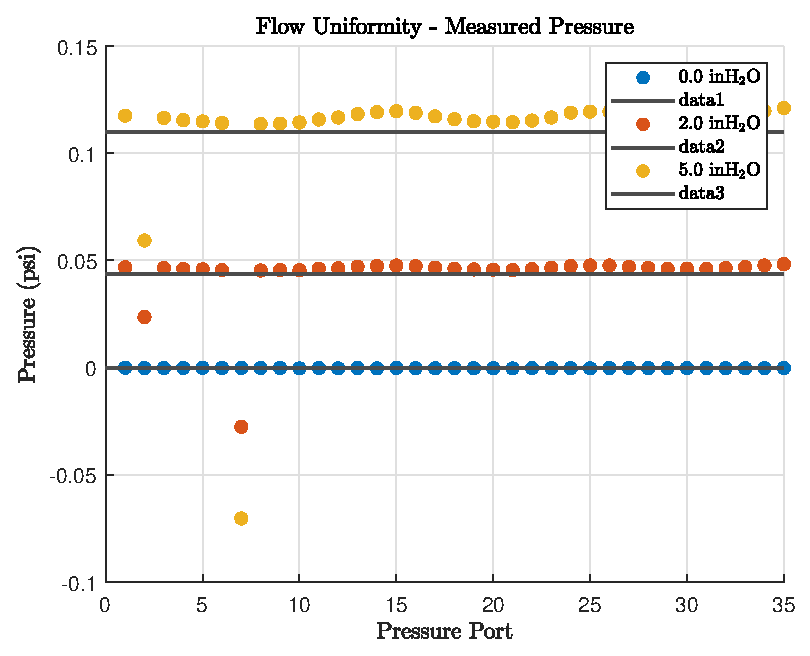
\includegraphics[width=0.8\textwidth]{Fig1.eps}
    \caption{Averaged pressure for three runs at dynamic pressures settings of 0.0inH$_2$O, 2.0inH$_2$O and 7.0 inH$_2$O. The black line is the average pressure for all pressure ports at a given dynamic pressure setting. The red rectangles mark points of interest. }
    \label{fig:fig1}
\end{figure}

\begin{figure}[H]
    \centering
    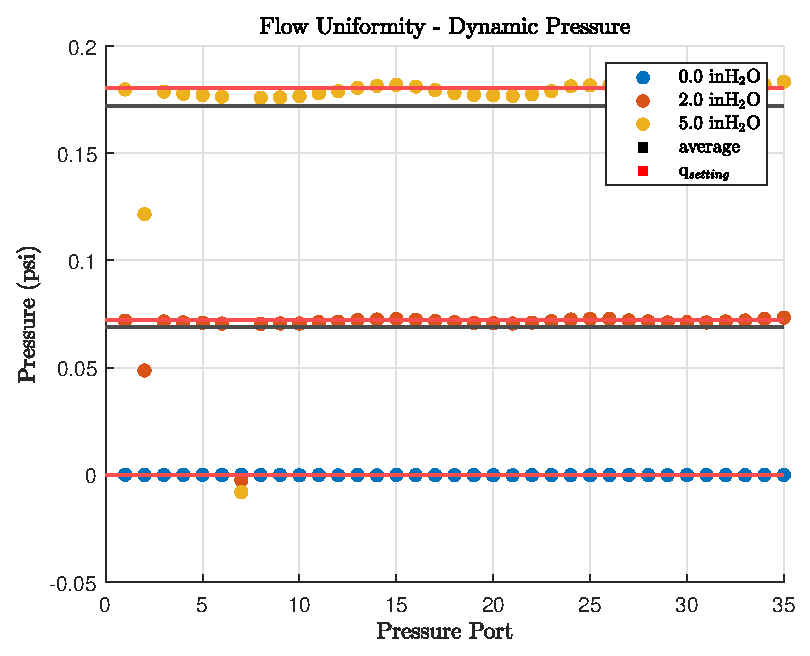
\includegraphics[width=0.8\textwidth]{Fig2.eps}
    \caption{Averaged measured dynamic pressure for three runs at indicated dynamic settings of 0.0inH$_2$O, 2.0inH$_2$O and 7.0 inH$_2$O. The black line is the average pressure for all pressure ports at a given dynamic pressure setting. The red rectangles mark points of interest.}
    \label{fig:fig2}
\end{figure}

\begin{figure}[H]
    \centering
    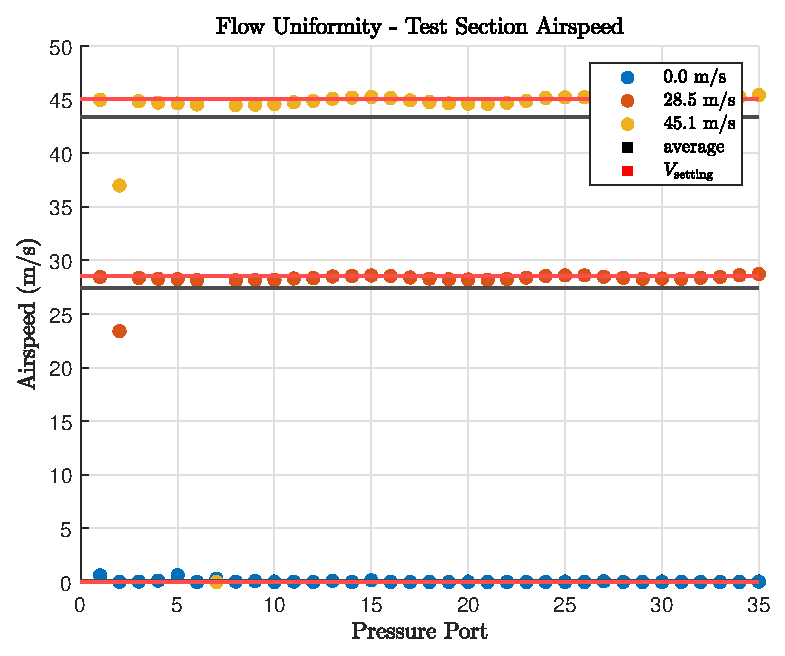
\includegraphics[width=0.8\textwidth]{Fig3.eps}
    \caption{Averaged measured airspeed for three runs at airspeeds settings of 0 m/s, ~28.5  m/s, ~45.1 m/s. The black line is the average airspeed for all pressure ports at a given airspeed setting. The red rectangles mark points of interest}
    \label{fig:fig3}
\end{figure}

\subsection{Dynamic Pressure Uniformity}
\begin{figure}[H]
    \centering
    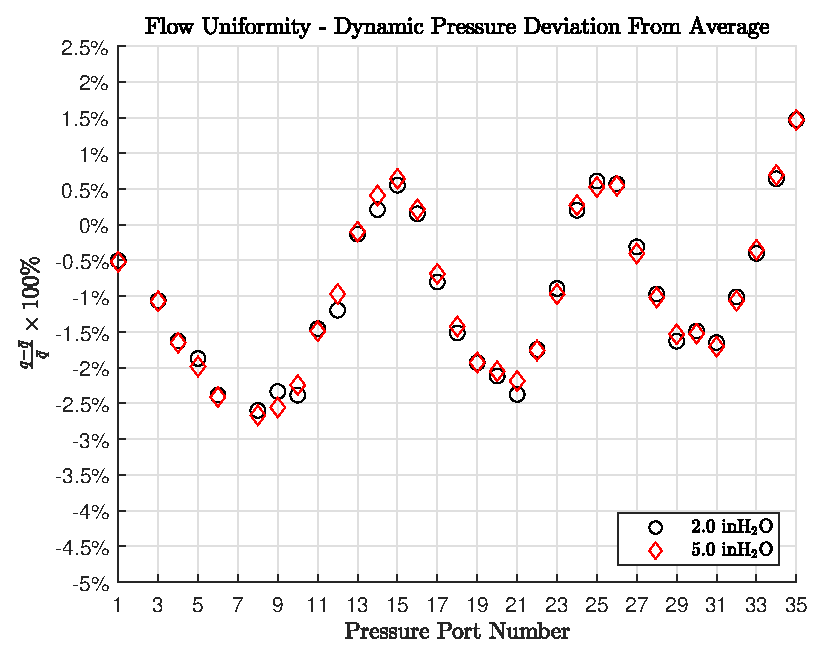
\includegraphics[width=0.8\textwidth]{Fig4.eps}
    \caption{Flow uniformity for dynamic pressure setting of 2 inH$_2$O and 5 inH$_2$O.}
    \label{fig:fig4}
\end{figure}

\begin{figure}[H]
    \centering
    \includegraphics[width=0.8\textwidth]{Fig5.eps}
    \caption{Flow uniformity for dynamic pressure setting of 2 inH$_2$O.}
    \label{fig:fig5}
\end{figure}

\begin{figure}[H]
    \centering
    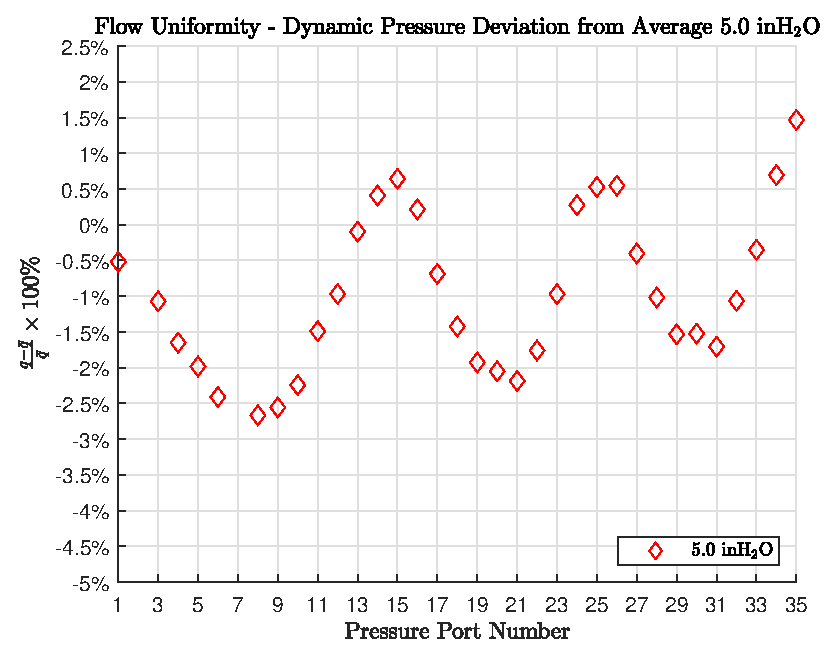
\includegraphics[width=0.8\textwidth]{Fig6.eps}
    \caption{Flow uniformity for dynamic pressure setting of 5 inH$_2$O.}
    \label{fig:fig6}
\end{figure}

\subsection{Airspeed Uniformity}
\begin{figure}[H]
    \centering
    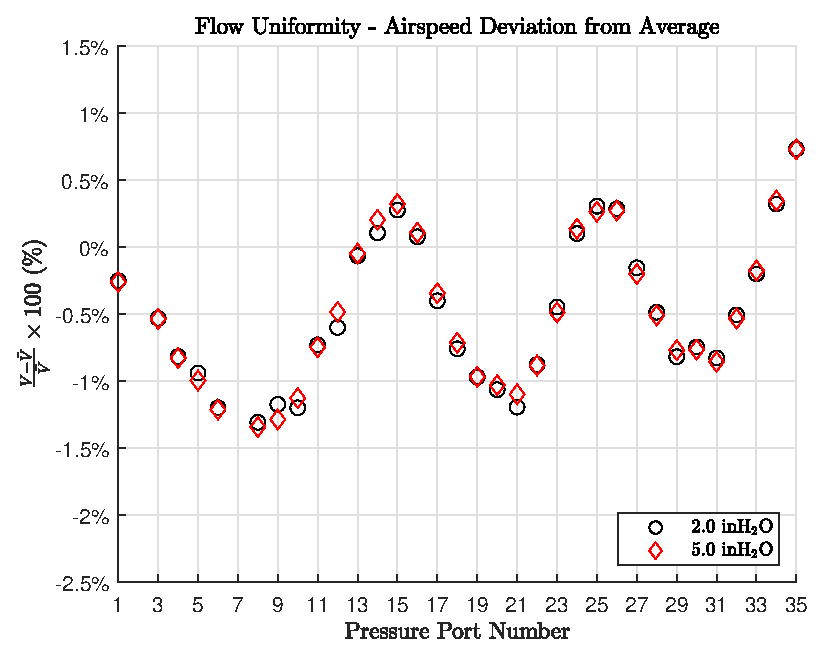
\includegraphics[width=0.8\textwidth]{Fig7.eps}
    \caption{Airspeed uniformity for dynamic pressure settings of 2 inH$_2$O and 5 inH$_2$O.}
    \label{fig:fig7}
\end{figure}

\begin{figure}[H]
    \centering
    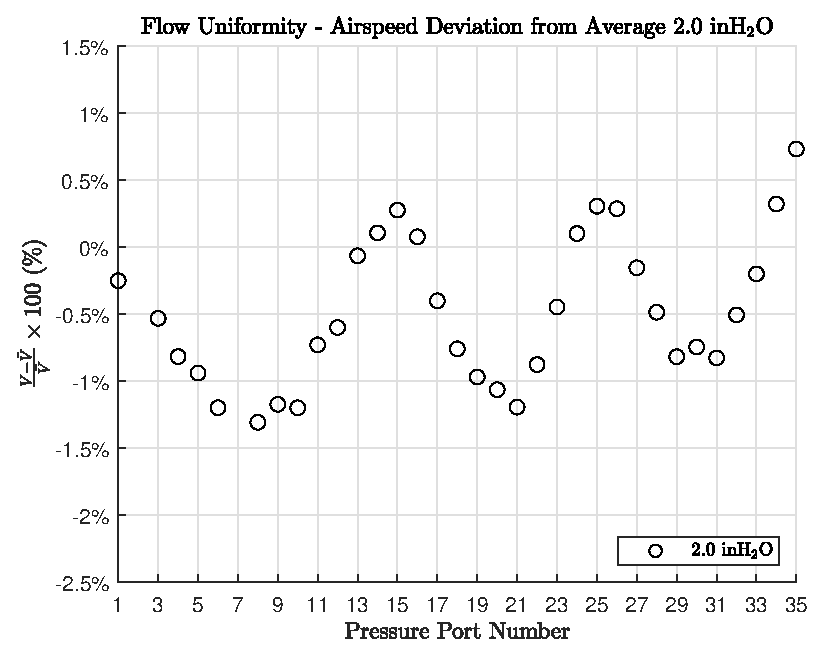
\includegraphics[width=0.8\textwidth]{Fig8.eps}
    \caption{Airspeed uniformity for dynamic pressure settings of 2 inH$_2$O.}
    \label{fig:fig8}
\end{figure}

\begin{figure}[H]
    \centering
    \includegraphics[width=0.8\textwidth]{Fig9.eps}
    \caption{Airspeed uniformity for dynamic pressure settings of 5 inH$_2$O.}
    \label{fig:fig9}
\end{figure}

\subsection{Dynamic Pressure Contours}
\begin{figure}[H]
    \centering
    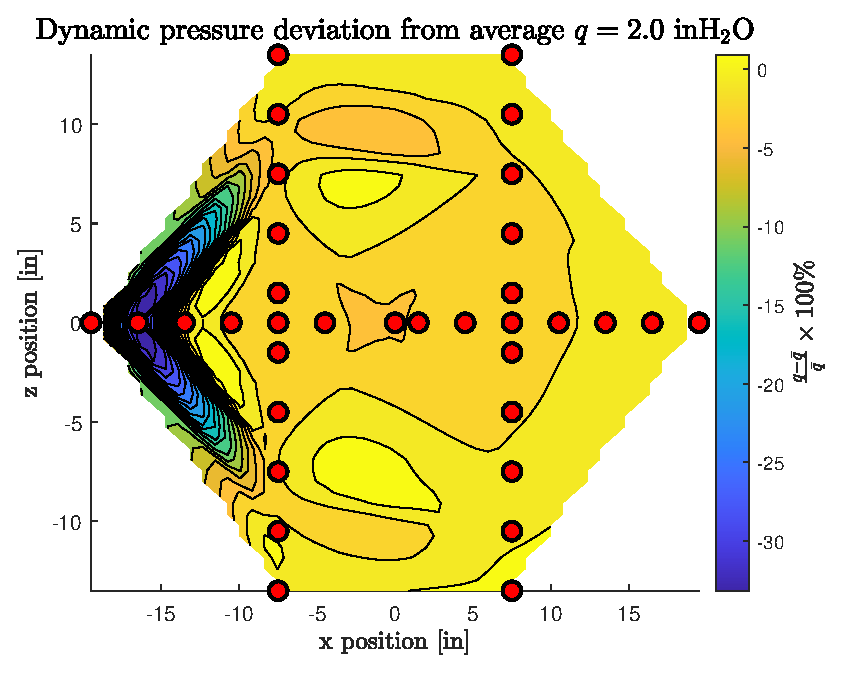
\includegraphics[width=0.8\textwidth]{Fig10.eps}
    \caption{Dynamic pressure fluctuation map for dynamic pressure setting of 2.0 inH$_2$O.}
    \label{fig:fig10}
\end{figure}

\begin{figure}[H]
    \centering
    \includegraphics[width=0.8\textwidth]{Fig11.eps}
    \caption{Dynamic pressure fluctuation map for dynamic pressure setting of 5.0 inH$_2$O.}
    \label{fig:fig11}
\end{figure}

\subsection{Airspeed Contours}
\begin{figure}[H]
    \centering
    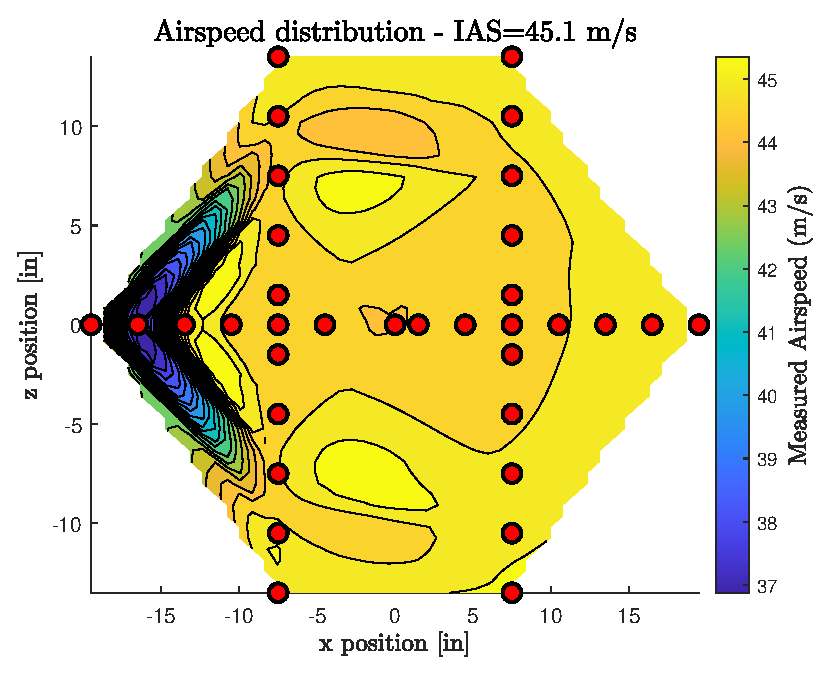
\includegraphics[width=0.8\textwidth]{Fig12.eps}
    \caption{Airspeed map for IAS 28.5 m/s.}
    \label{fig:fig12}
\end{figure}

\begin{figure}[H]
    \centering
    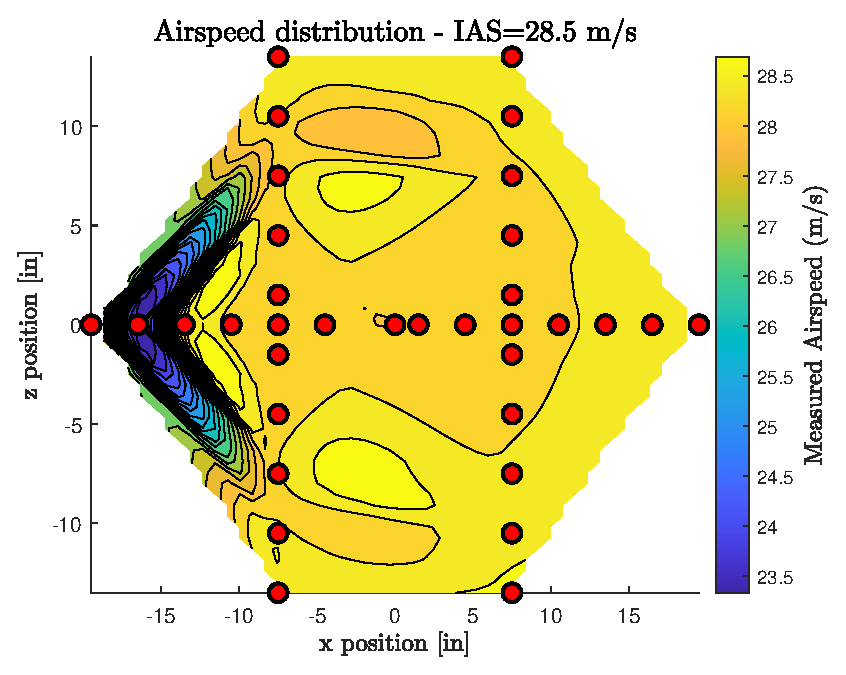
\includegraphics[width=0.8\textwidth]{Fig13.eps}
    \caption{Airspeed map for IAS 45.1 m/s.}
    \label{fig:fig13}
\end{figure}

\subsection{Convergence Test}
\begin{figure}[H]
    \centering
    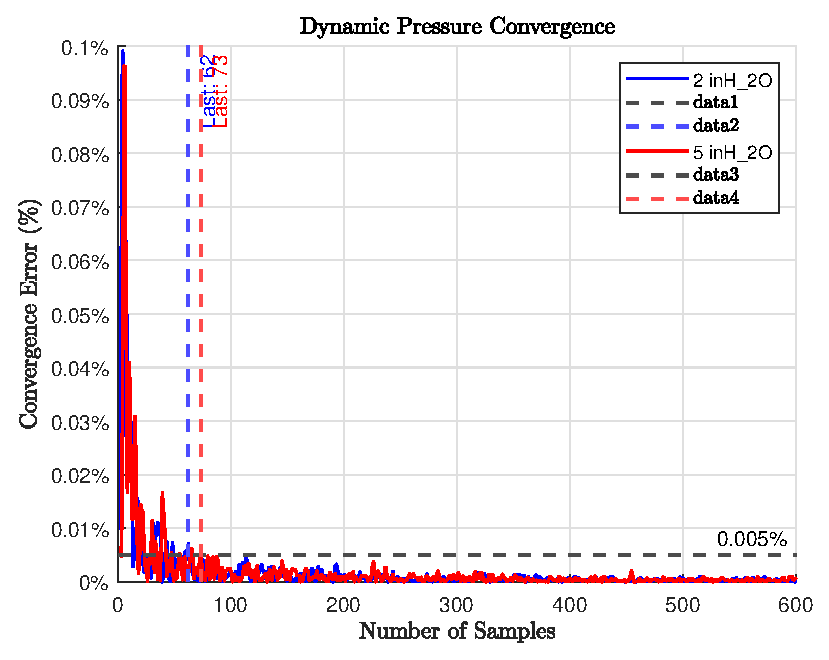
\includegraphics[width=0.8\textwidth]{Fig14.eps}
    \caption{Convergence test over 600 samples at 2 inH$_2$O and 5 inH$_2$O.}
    \label{fig:fig14}
\end{figure}

\begin{table}[H]
    \centering
    \caption{Convergence Results for Dynamic Pressure}
    \begin{tabular}{l c}
        \toprule
        \textbf{Test Condition} & \textbf{Samples Required for Convergence} \\
        \midrule
        2 inH$_2$O  & 62 Samples \\
        5 inH$_2$O  & 73 Samples \\
        \bottomrule
    \end{tabular}
    \label{tab:convergence}
\end{table}


\section{Discussion}

The negative pressure readings at Port \#7 are an expected behavior due to flow separation occurring at that location. As the Indicated Airspeed (IAS) increases, the velocity difference between the main flow and the recirculating region grows, leading to a further reduction in pressure according to Bernoulli’s principle.

The non-zero average pressure reading for IAS = 0 may be attributed to sensor noise, ambient pressure fluctuations, or minor errors in zeroing the pressure transducers. Since the dynamic pressure is computed based on the differential pressure readings, any offset in the baseline measurement could introduce small deviations in Figures 2 and 3. However, these deviations are likely within the acceptable experimental error margins.

The pressure and airspeed measurements at Port \#34 exhibit deviations from the expected average values. This could result from localized turbulence, obstruction, or slight misalignment of the Pitot tube. While such discrepancies influence flow uniformity measurements, they do not necessarily invalidate the experiment but highlight the importance of accounting for anomalies and potential test section irregularities.

An increase in air temperature was observed with increasing airspeed. This phenomenon occurs due to adiabatic heating caused by air compression, as well as frictional heating from the tunnel walls. Additionally, interaction between the test section and the surrounding environment contributes to the observed temperature rise.

To mitigate temperature variations, pre-conditioning the incoming air, implementing heat exchangers, or maintaining a controlled test environment can be effective strategies. Reducing test duration and ensuring proper ventilation can further help regulate temperature fluctuations.

The rise in temperature affects both the IAS calculation and the unit Reynolds number. As temperature increases, air density decreases, altering the dynamic pressure readings. Since the Reynolds number is defined as:

\begin{equation}
Re = \frac{\rho V L}{\mu}
\end{equation}

a reduction in air density leads to a lower Reynolds number, affecting the boundary layer behavior and overall flow characteristics in the test section.


\section{Conclusion}
This experiment analyzed the flow uniformity in a low-speed wind tunnel using a total pressure rake. Dynamic pressure and airspeed variations followed expected trends, validating Bernoulli’s equation. Negative pressure at port \#7 and deviations at port \#34 suggested localized flow disturbances. Temperature effects on IAS and Reynolds number were observed, emphasizing the need for environmental control. Convergence analysis showed 62 and 73 samples were required for 2 inH$_2$O and 5 inH$_2$O, respectively. The study reinforced wind tunnel testing principles and the importance of data reduction techniques.


\section*{Acknowledgments}
The author would like to thank Dr. Xiaofeng Liu for his guidance and Teacher's Assistant Andrew Balolong for assistance during the experiment.

\section{Appendix}
\appendix
\section{Sample Data}

The following table presents a portion of the raw experimental data collected for the \texttt{0inH2O.csv} dataset. Due to space limitations, only the first few rows are shown as a representative sample.

\begin{table}[H]
    \centering
    \caption{Excerpt from \texttt{0inH2O.csv} dataset}
    \label{tab:sample_data}
    \scriptsize % Reduce font size to fit more data
    \csvautotabular{0inH2O.csv} % Automatically format CSV data as a table
\end{table}

The complete dataset consists of 600 samples recorded across 37 pressure ports, along with total and static pressure measurements. This data was used for further analysis and flow characterization.

\section{MATLAB Code}
\lstinputlisting[language=Matlab, caption={MATLAB Code for Data Analysis}]{AE303_Lab2.m}

\end{document}
